
\section{Design}
\label{sec:design}

In this section we begin with a system overview of \texttt{Parikshan}. 
We then explain how it inserts test cases, into the test harness, and finally we explain how a user can use the \texttt{Parikshan} api to insert test cases in the test harness.

\begin{figure*}[t]
  \begin{center}
    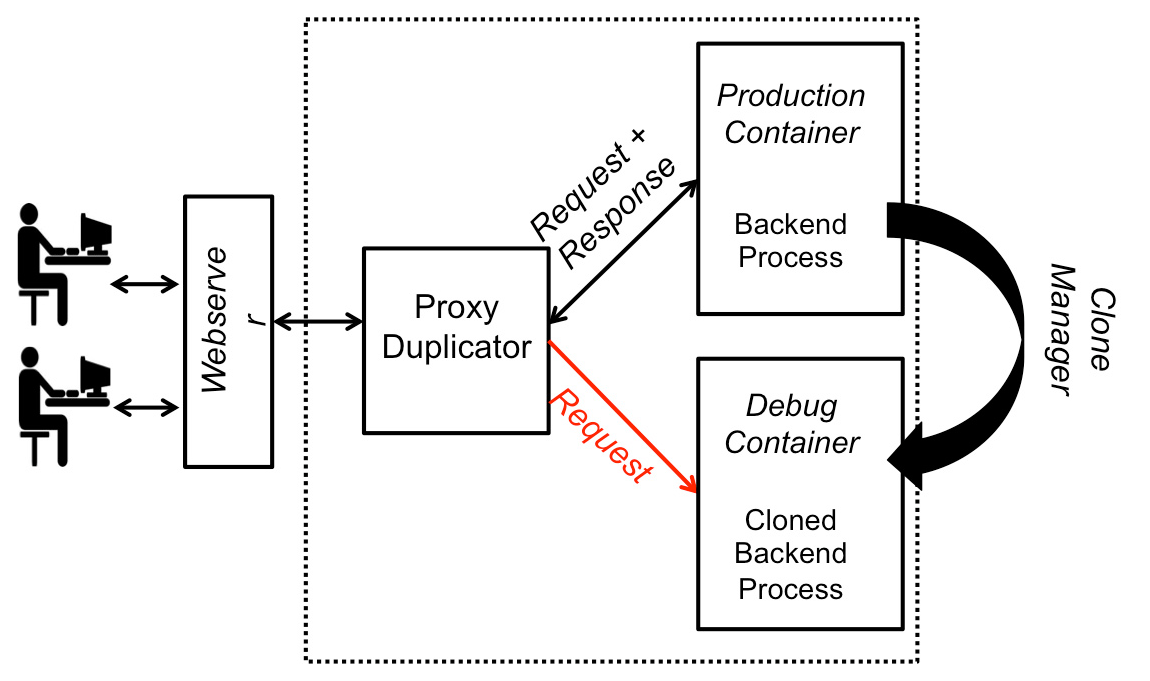
\includegraphics[width=0.8\textwidth]{figs/workflow2.eps}
    \caption{Backend wrapped around with Parakishan Run-time}
    \label{fig:workflow}
  \end{center}
\end{figure*}

\subsection{How does cloning work?}

While the focus of our work is not to support VM/Container migration, or to make changes to the hypervisor, we need to tweak the way typical hypervisors offer live migration for our purposes.
Before moving further we fish to clarify that instead of the typical live migration supported by hypervisors, \textit{Parikshan} requires a clone of the production container. 
In contrast with live migration, where a container is copied to a target destination, and then the original container is destroyed, the cloning process requires both containers to be actively running, and be still attached to the original network.
This cloning requires some tweaking, and modification in both how compute migration is handled, and especially how the network migration is handled. 

To understand cloning in our context, one must first understand how live migration works. 
Live migration refers to the process of moving a running virtual machine, guest os or container from one host node(physical machine) to another, without disconnecting any client or process running within the machine. 
There are several variants of live migration, some of which require a short suspend time, while others are able to seamlessly transfer without any noticeable down-time by the user.
In general the process involves the following steps: (1) Firstly, the copy is initiated by a pre-copy memory migration, where the underlying hypervisor copies all the memory pages from the source to the destination. (2) Once pre-copy phase is finished, the VM is temporarily suspended, and all memory pages including live memory pages are transferred to the target node. 
Once all memory pages have been transferred the target container is restarted. 
To reduce the down-time memory pages are transferred probabiliticly based on priority, and incase a page is not found a network fault is generated which executes a fetch from the original VM.
Network migration is managed by the IAAS which publishes the same MAC address for the copied VM. 
Since the identity of the target container remains the same, the IAAS is able to give it same IP Address, and network traffic is rerouted after the identity is published in the network.

Instead of Live Migration, in Live Cloning, we do not suspend operations of the source container, rather we allow the container to keep executing in both production and test locations.
The more tricky aspect is that there are two containers with the same identities in the network and application domain. 
Hence the same network identifier should map to two seperate addresses.
Further a packet level sniffer or mirror port would keep the same buffer and potentially timeout.
To allow for some load-balancing and an application aware buffer, we went for a web application level proxy server to duplicate traffic to both containers. 
Further in this section we explain how we deal with these challenges.

\subsection{System Overview}

Each instance of \textit{Parikshan} can target only one tier at a time.
Multiple instances of \textit{Parikshan} can be orchestrated together especially when it's required for integration testing or cross tier results need to be correlated.

To begin with let us look at a simple example of client webserver with a database server as the backend, where the test harness needs to be applied on the backend.
The architecture can be divided into two parts: (1) A Proxy Network Duplicator, (2) container clone manager

\begin{itemize} 

\item \textbf{Proxy Network Duplicator} As described earlier an important aspect of live cloning is that we have two replicas which share the same identity.
Clearly two containers cannot share the same network identity. 
While we do not have strong consistency measures, in order for both containers to execute they must receive the same input.
This can be achieved in multiple ways, the easiest would be a packet level tap device or a hardware switch which does port mirroring. 
These are both pretty common, and are blackbox and do not require much configuration.
However, such port mirroring solution gives us minimal control on the traffic going to our test container.
The production and test-container may execute at varying speeds which will result in them being slightly out of sync.
Additionally we need to accept responses from both servers and drop all the traffic coming from the test-container, while still mantaining an active connection with the client.
Hence a layer 2 level network solution is not possible as some context of the address and state are required

We have implemented our duplicator in two modes: (1) at TCP level, (2) at application level.
The TCP level duplicator is configured with the client facing ip address (hence it becomes  a a proxy), and essentially works as a socket reader/writer which reads incoming TCP streams and writes these streams to two different socket connections for the production and test containers.


\item \textbf{Clone Manager} 

\end{itemize}
